\documentclass[pdf,fyma2]{beamer}
\usepackage{caption}
\usepackage[linesnumbered,ruled,onelanguage,commentsnumbered,longend]{algorithm2e}
\usetheme{CambridgeUS}
\definecolor{myNewColorA}{RGB}{139,0,0}

\captionsetup{labelformat=empty}

\title{Graph algorithms}
\author{David Svaty}
\institute{ Faculty of Information Technology, BUT }
\date{\today}

\titlegraphic{
\includegraphics[height=2cm]{img/vut.png}} 

\begin{document}
    
\frame{\titlepage}

\begin{frame}
    \frametitle{What is a graph}
    
    \begin{itemize}
        \item Non-linear data structure
        \pause
        \item Consists of vertices and edges
        \pause
        \item Vertices are nodes and edges connect them
        \pause
        \item Denoted by $G(E,V)$ 
    \end{itemize}
\end{frame}

\begin{frame}
    \frametitle{Graph example}
    \begin{figure}
        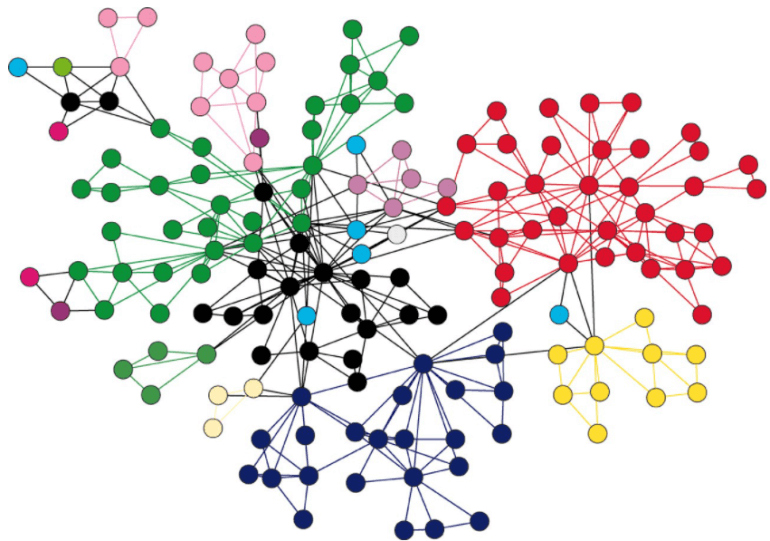
\includegraphics[width=170px]{img/graph-algorithms1.png}
        \caption{Example of a graph. Graph consists of nodes connected by lines.}
    \end{figure}
\end{frame}

\begin{frame}
    \frametitle{Examples of graph algorithms}
    \begin{itemize}
        \item Breadth-first search
        \pause
        \item Depth-first search
        \pause
        \item Shortest path
        \pause
        \item Minimum spanning tree 
    \end{itemize}    
\end{frame}

\begin{frame}
    \frametitle{Dijkstra's algorithm}

    \begin{columns}

    \begin{column}{0.5\textwidth}
        \begin{itemize}
            \item Used in weighted graphs
            \item Finds the shortest path in between nodes
        \end{itemize}
    \end{column}
    
    \begin{column}{0.5\textwidth}
        \begin{figure}
            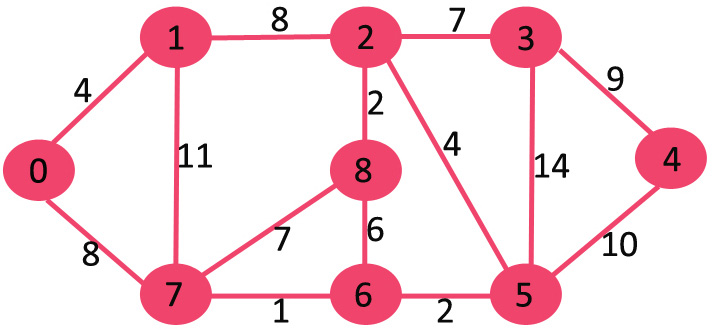
\includegraphics[width=\textwidth]{img/dijsktra_graph.jpg}
            \caption{Example of a weighted graph}
        \end{figure}
    \end{column}
    
    \end{columns}
    
\end{frame}

\begin{frame}
    \frametitle{Time complexity}
\end{frame}

\begin{frame}
    \frametitle{Pseudocode}
    
    \begin{center}
    \scalebox{0.65}{
    \begin{minipage}{0.7\linewidth}
        
    \begin{algorithm}[H]
        \SetAlgoNoLine
        \SetNlSty{}{}{:\enspace}
        \Indp
        \KwIn{G,V}
        \KwOut{distance[ ], previous[ ]}

        \ForEach{vertex V in G}{
            $distance[V] \leftarrow \inf$ \\
            $previous[V] \leftarrow null$ \\
            \If{V $\neq$ S}{$add\,V\,to\,Priority\,Queue\,Q$}
            $distance[S] \leftarrow 0$ \\
        }

        
        \While{Q is not empty}{
            $U \leftarrow Extract\,MIN\,from\,Q$ \\
            \ForEach{unvisited neighbour V of U}{
                $tempDistance \leftarrow distance[u] + edge\_weight(U,V)$ \\
                \If{tempDistance $<$ distance[V]}{
                    $distance[V] \leftarrow tempDistance$ \\
                    $previous[V] \leftarrow U$
                }
            }
        }

        \Return{distance[ ], previous [ ]}
    \end{algorithm}

    \end{minipage}
    }
    \end{center}
\end{frame}

\begin{frame}
    \textcolor{myNewColorA}{\Huge{\centerline{Thank you for your attention}}}
\end{frame}

\end{document}